\section{Introduction}
%\subsection{Confidence of Identification}

%\subsection{Alkylresorcinol Metabolism Pathway}
%includes three steps: 
%(1) a cytochrome P450-mediated $\omega$-oxidation of the alkyl side chain to form hydroxylated ARs, 
%(2) further oxidation of the hydroxylated intermediates to generate carboxylated ARs, and 
%(3) $\beta$-oxidation of the side chain to produce hydrophilic metabolites (Figure 1).14 Ross et al. 

%first reported 3,5-dihydroxybenzoic acid (3,5-DHBA) and 3- (3,5-dihydroxyphenyl)propanoic acid (3,5-DHPPA) as the major AR metabolites in humans in 2004.11 Several studies have shown that both 3,5-DHBA and 3,5-DHPPA had longer apparent half-lives (10-12 h) than their parent ARs, indicating they have the potential to reflect longer term WG wheat and rye intake.

%However, 3,5-DHBA and 3,5-DHPPA are not unique to ARs and have been reported from other food sources.15

%\subsection{Partition Coefficient and Its Predictions}
%	The hydrophobicity of an analyte molecule will be the primary indicator as to the retentivity in
%reversed phase HPLC. Hydrophobicity is often expressed as Log P which is a measure of the way
%an analyte (in its neutral form) partitions between two immiscible solvents (usually octanol and
%water) under standard conditions (Equation 1). The higher the value of Log P (between –1 and +1)
%the more hydrophobic the molecule.

\section{Materials and Methods}
	\subsection{\textit{In vitro} glucuronidation}
	\cite{Liu1984}
	%\subsection{Glucurnadase experiments}
	
	\subsection{Bioinformatics Tools and Software}
	Partition coefficient (logP and ClogP) was predicted by ChemDraw. 
	MS\textsuperscript{2} spectra was predicted by CFM-ID 3.0\cite{metabo9040072}.
	
	\subsection{MS/MS}
	
	
\section{Results}
\subsection{Summary of Identification}
N metabolites were identified. Within them, Ni as level I, Nii as level II. 
\begin{table}[h!]
\centering
\scalebox{0.80}{
\begin{tabular}{|c|c|c|c|c|c|c|}
	\hline 
	No. & m/z & \makecell{RT\\(Quad)}& \makecell{RT\\(Bi)} & MS/MS & Annotation & \makecell{Suggested\\Compound} \\ 
	\hline 
	& 263.016 & 5.26 & 3.31 &  & &  \\ 
	\hline 
	& 329.0582 & 2.54&0.97   &  & [M-H]\textsuperscript{-}& 3,5-DHBA glucuronate\\ 
	\hline
	& 329.0582 & 3.51&1.12   &  &[M-H]\textsuperscript{-} & 3,5-DHBA glucuronate\\ 
	\hline 
	& 253.9750 & 3.58 & 1.37 &  &[M-H]\textsuperscript{-} & 3,5-DHBA sulfate \\ 
	\hline 
	& 210.0411 &  & 1.48 &  &[M-H]\textsuperscript{-} & 3,5-DHBA glycine \\ 
	\hline
	& 153.0187 & 1.18 & 1.88 & 109.029 &[M-H]\textsuperscript{-} & 3,5-DHBA\\ 
	\hline	
	& 357.0898 & 4.24  & 1.91 &  &[M-H]\textsuperscript{-} & \makecell{3,5-DHPPA\\glucuronate}\\ 
	\hline
	& 715.1716 & 4.24  & 1.91 &  &[2M-H]\textsuperscript{-} & \makecell{dimer of \\3,5-DHPPA glucuronate}\\ 
	\hline
	& 261.0077 & 4.32  & 2.10 &  &[2M-H]\textsuperscript{-} & \makecell{3,5-DHPPA sulfate}\\ 
	\hline		
\end{tabular} }
\end{table}
	
\subsection{Predicted logP value of AR metabolites}
\begin{table}[h!]
\scalebox{0.78}{
	\begin{tabular}{|c|c|c|c|c|c|c|}
		\hline 
		\multicolumn{1}{|c|}{}&\multicolumn{3}{c}{ChemDraw}&\multicolumn{3}{|c|}{ClogP}\\
		\hline
		&M&[M+GluA+H]\textsuperscript{+}&[M+SO3+H]\textsuperscript{+}&M&[M+GluA+H]\textsuperscript{+}&[M+SO3+H]\textsuperscript{+}  \\ 
		\hline 
		3,5-DHPPTA& 2.01 & 0.75 &0.55  &1.48  & -0.44 & 0.10 \\
		\hline
		3,5-DHPPA& 1.17 & -0.09 & -0.36 & 0.57 &-1.34  &-0.81  \\
		\hline
		3,5-DHBA& 0.81 & -0.45 & -1.00 & 0.99 &-1.07  &-0.54  \\
		\hline
		3,5-DHBA glycine& -0.34 &-1.60  & -2.34 & -0.24 & -2.29 & -1.75 \\ 
		\hline 
	\end{tabular}} 
\end{table}
The general pattern for metabolites are eluting late when chain length increases.

\subsection{\textit{in-vitro} glucuronadation of 3,5-DHBA}
3,5-DHBA has 3 active sites to be glucuronated. The products could be mono-, di- or tri- glucuronate (Figure-\ref{fig:35-dhba-all}).

\begin{tabular}{|c|c|c|}
	\hline 
	RT & m/z & Annotation \\ 
	\hline 
	2.78 & 329.05 & \makecell{[3,5-DHBA + GluA - H]\textsuperscript{-}\\(glucuronated at carboxylic acid hydroxyl group)} \\ 
	\hline 
	3.97 & 329.05 & \makecell{[3,5-DHBA + GluA - H]\textsuperscript{-}\\ (glucuronated at benzene hydroxyl group)} \\ 
	\hline 
	3.6 & 252.04 & [3,5-DHBA + 2GluA - 2H]\textsuperscript{2-} \\ 
	\hline 
	7.34 & 339.55 & [3,5-DHBA + 3GluA - 2H]\textsuperscript{2-}\\ 
	\hline 
\end{tabular} 
\begin{figure}[h!]
	\centering
	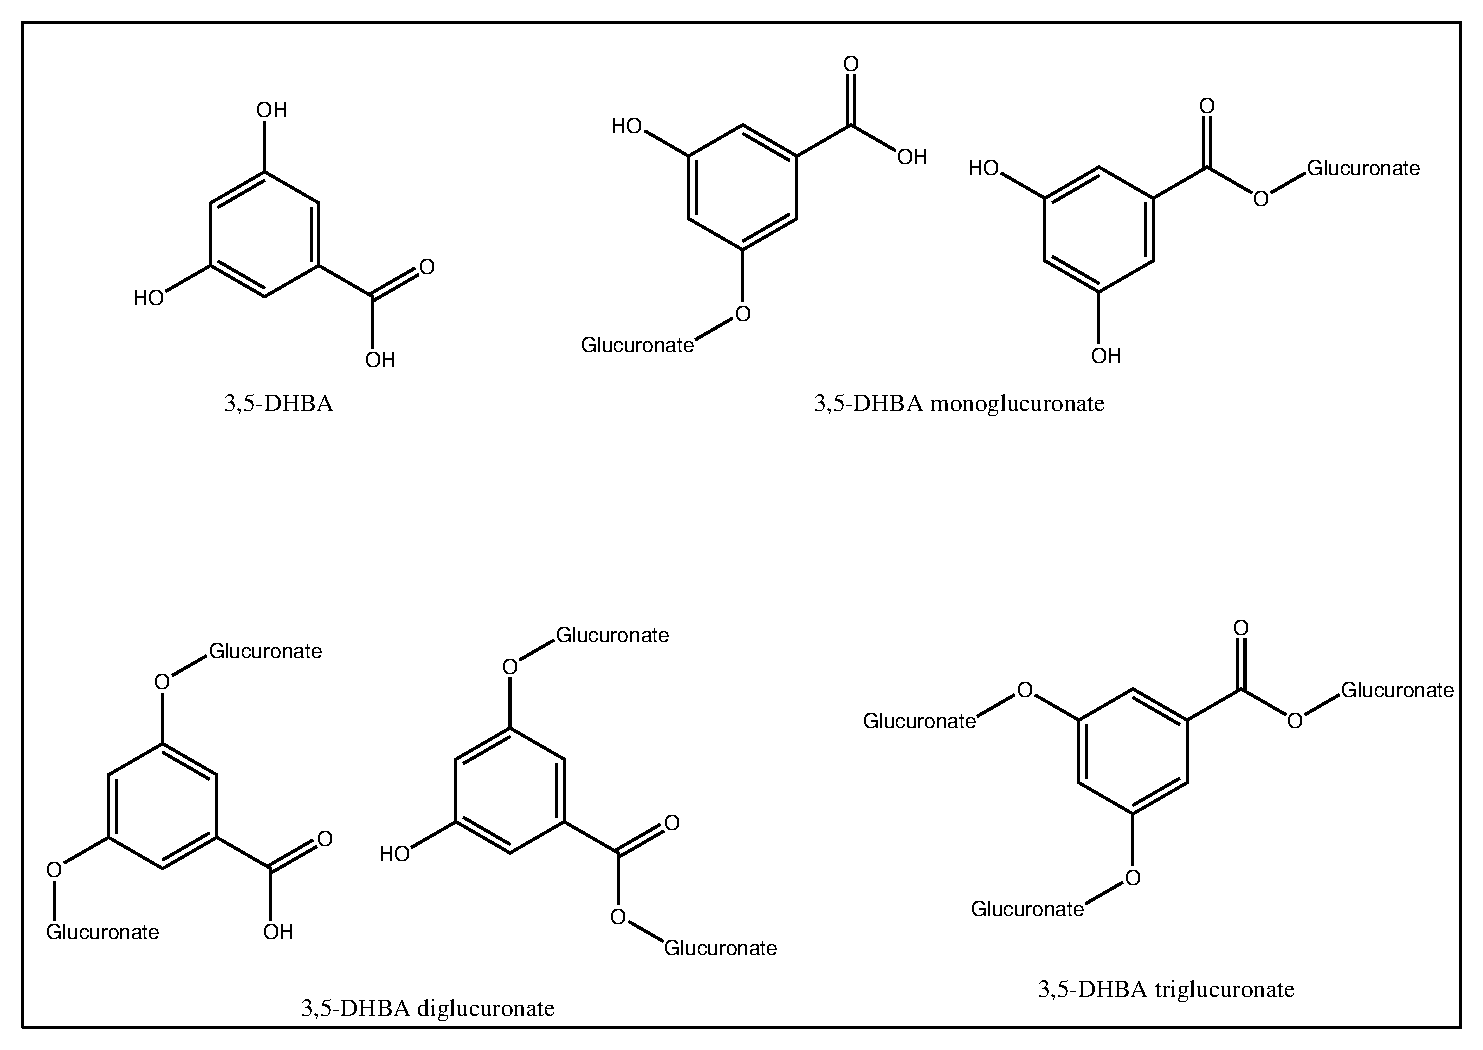
\includegraphics[width=1\linewidth]{picture/3,5-DHBA-glca-all}
	\caption{3,5-DHBA}
	\label{fig:35-dhba-all}
\end{figure}


\subsubsection{3,5-DHBA monoglucuronate}
3,5-DHBA mono-glucuronate exists 2 theoretical possibilities. Because position 3 and 5 are equal. The difference is phenol group or hydroxyl group sitting on carboxyl group be substituted.

Fragment 109 and 137 are specific for glucuronation reaction happening in carboxylic acid or beneze ring. Based on their predicted ClogP value and fragment 109 and 137 ratio. Finally, we confirmed RT 2.78 should be 3-glucuronate-5-hydroxyl-benzoic acid, RT 3.97 should be A. something in between, we have no idea.


\begin{figure}[h!]
	\centering
	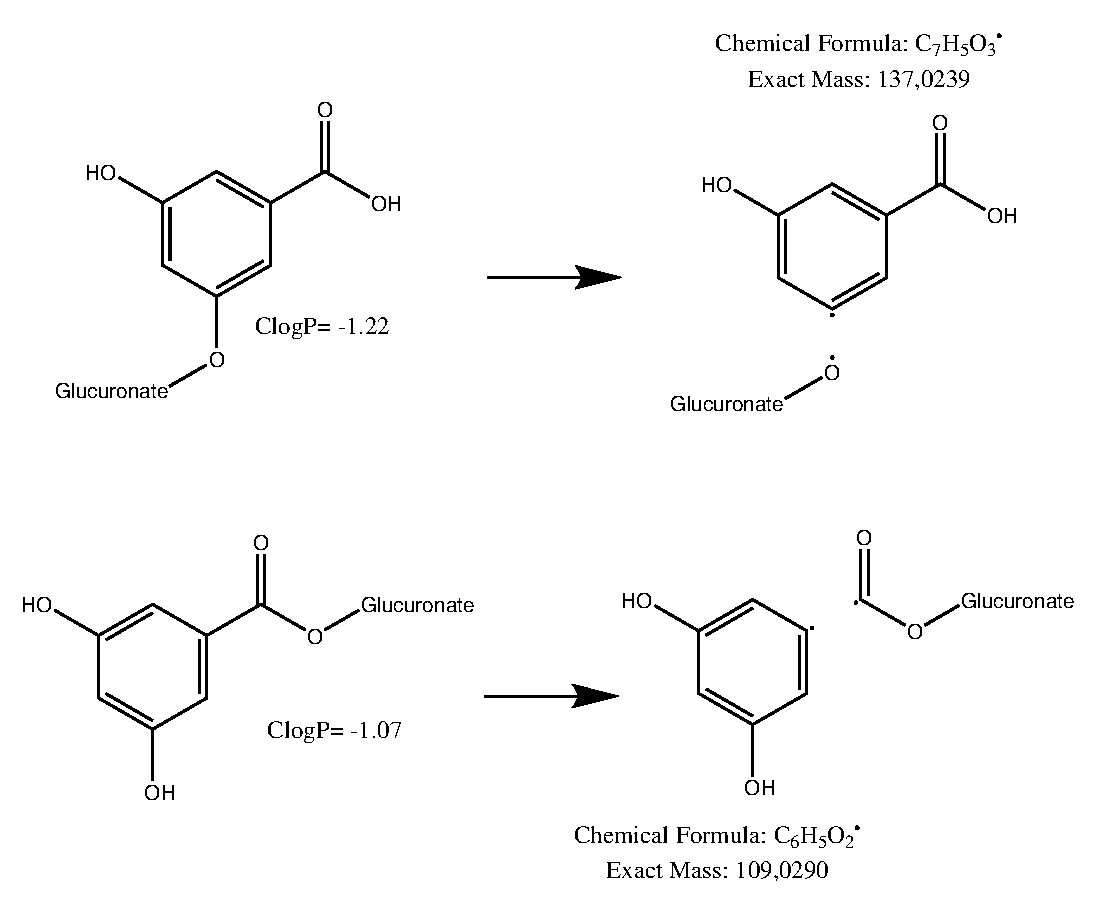
\includegraphics[width=1\linewidth]{picture/3,5-DHBA-glca-mono}
	\caption{Fragmentation of 3,5-DHBA monoglucuronate}
	\label{fig:35-dhba-glca-mono}
\end{figure}

\begin{table}[h!]
	\centering
\begin{tabular}{|c|c|c|c|}
	\hline 
	RT & \makecell{Intensity of\\ 109} & \makecell{Intensity of\\ 137} & \makecell{Ratio of \\109:137} \\ 
	\hline 
	2.78 & 195 & 1.58e3 & 1.23e-1 \\ 
	\hline 
	3.08 & 1.48e3 & 27.8 & 52.23 \\ 
	\hline 
	3.97 & 2.79e4 & 34.7 & 804 \\ 
	\hline 
\end{tabular} 
\caption{3,5-DHBA monoglucuronate}
\label{tab:35-dhba-monoglucuronate}
\end{table}

\subsubsection{3,5-DHBA diglucuronate and triglucuronate}
3,5-DHBA di- and tri- glucuronates were also detected.
3,5-DHBA di-glucuronate has 2 possible isomers. But they were not confirmed here.

3,5-DHBA tri-glucuronate does not have isomers. It is detected as [M+3 GluA-2H]2-.

\subsection{3,5-DHBA sulfate}

\subsection{Identifications of alkylresorcinol (AR) metabolites}

\section{Conclusion}


\section{Discussion}